\chapter{Implementation and Individual Contributions}

This chapter presents the complete implementation details of the Electronic Health Record (EHR) System, organized by the individual contributions of each team member. Each section describes the components built, the containers hosted, the technical methodology, relevant pseudo code, and application walkthrough.

%% ════════════════════════════════════════════════════════════════════════════
%% SECTION 1: ANKIT
%% ════════════════════════════════════════════════════════════════════════════

\section{Ankit Chaudhari (25CSM2R03): Infrastructure Architect \& Swarm Master}

\subsection{Role Overview}
Ankit is responsible for the core network infrastructure, including Docker Swarm orchestration, deployment automation, cryptographic material management, and the Manager Governance Portal. He operates PC1, the Swarm Manager node.

\subsection{Containers Hosted on PC1}

\begin{table}[h]
\centering
\caption{PC1 Container Inventory (Ankit Chaudhari)}
\label{tab:ankit_containers}
\begin{tabular}{|l|l|p{6cm}|}
\hline
\textbf{Container} & \textbf{Image} & \textbf{Purpose} \\
\hline
Fabric CA & hyperledger/fabric-ca:1.5 & Root Certificate Authority for PKI \\
\hline
Raft Orderer & hyperledger/fabric-orderer:2.5 & Transaction ordering and block creation \\
\hline
Peer0 & hyperledger/fabric-peer:2.5 & Anchor peer for Org1MSP \\
\hline
CouchDB0 & couchdb:3.3.2 & State database for Peer0 \\
\hline
Manager Portal & Node.js / React (Vite) & Governance UI for identity provisioning \\
\hline
\end{tabular}
\end{table}

\subsection{Docker Swarm Orchestration}

The deployment leverages Docker Swarm's stack-based service definitions. Each Fabric component is defined as a separate Docker Compose stack YAML file:

\begin{itemize}
    \item \texttt{compose/stack-ca.yaml} — Fabric CA service
    \item \texttt{compose/stack-orderer.yaml} — Raft Orderer service
    \item \texttt{compose/stack-peer0.yaml} — Peer0 and CouchDB0
    \item \texttt{compose/stack-peer1.yaml} — Peer1 and CouchDB1 (deployed to PC2)
    \item \texttt{compose/stack-peer2.yaml} — Peer2 and CouchDB2 (deployed to PC3)
\end{itemize}

Swarm placement constraints ensure containers run on the correct physical node:
\begin{lstlisting}[language=bash, caption={Placement Constraint Example (stack-peer1.yaml)}]
deploy:
  placement:
    constraints:
      - node.labels.role == worker2
\end{lstlisting}

\subsection{Deployment Automation (\texttt{deploy.sh})}

The \texttt{deploy.sh} script automates the entire network lifecycle. It is a single-command deployment tool that performs the following steps:

\begin{algorithm}[H]
\caption{One-Click Network Deployment}
\label{alg:deploy}
\begin{algorithmic}[1]
\Procedure{Deploy}{}
    \State \textbf{Step 1:} Stop all existing Docker stacks and kill running application processes
    \State \textbf{Step 2:} Wipe old ledger data volumes on PC1, PC2, and PC3 (via SSH)
    \State \textbf{Step 3:} Start the IPFS daemon on PC1
    \State \textbf{Step 4:} Package the EHR chaincode into \texttt{ehr.tar.gz}
    \State \textbf{Step 5:} Deploy the Fabric CA and Orderer stacks on PC1
    \State \textbf{Step 6:} Create the channel genesis block (\texttt{mychannel.block})
    \State \textbf{Step 7:} Sync crypto-materials and channel block to PC2 and PC3 via SCP
    \State \textbf{Step 8:} Deploy Peer0, Peer1, and Peer2 stacks across the Swarm
    \State \textbf{Step 9:} Join all three peers to \texttt{mychannel}
    \State \textbf{Step 10:} Install, approve, and commit the chaincode lifecycle
    \State \textbf{Step 11:} Import wallet identities for the API Gateway
    \State \textbf{Step 12:} Start the Node.js backend and all React frontend portals
    \State \textbf{Step 13:} Seed initial dummy data for demonstration
\EndProcedure
\end{algorithmic}
\end{algorithm}

\subsection{Cryptographic Material Distribution}

A critical challenge in multi-node Fabric deployment is ensuring all worker nodes possess the correct MSP (Membership Service Provider) credentials before their peer containers start. The \texttt{deploy.sh} script solves this via automated SCP transfers:

\begin{lstlisting}[language=bash, caption={Crypto-Material Sync to Worker Nodes}]
# Sync crypto-config, channel block, and chaincode to PC2
scp -r crypto-config/ rajput_mt@100.83.121.98:~/fabric-network-swarm/
scp mychannel.block   rajput_mt@100.83.121.98:~/fabric-network-swarm/
scp ehr.tar.gz        rajput_mt@100.83.121.98:~/fabric-network-swarm/

# Sync to PC3
scp -r crypto-config/ ronit@100.117.138.55:~/fabric-network-swarm/
scp mychannel.block   ronit@100.117.138.55:~/fabric-network-swarm/
scp ehr.tar.gz        ronit@100.117.138.55:~/fabric-network-swarm/
\end{lstlisting}

\subsection{Manager Portal}

The Manager Portal is a React-based governance interface that allows hospital administrators to:

\subsubsection{Functional Procedures}

\textbf{1. Manager Dashboard \& Overview:}
The dashboard acts as the primary landing page, giving the administrator a high-level view of system modules.
\begin{figure}[h]
    \centering
    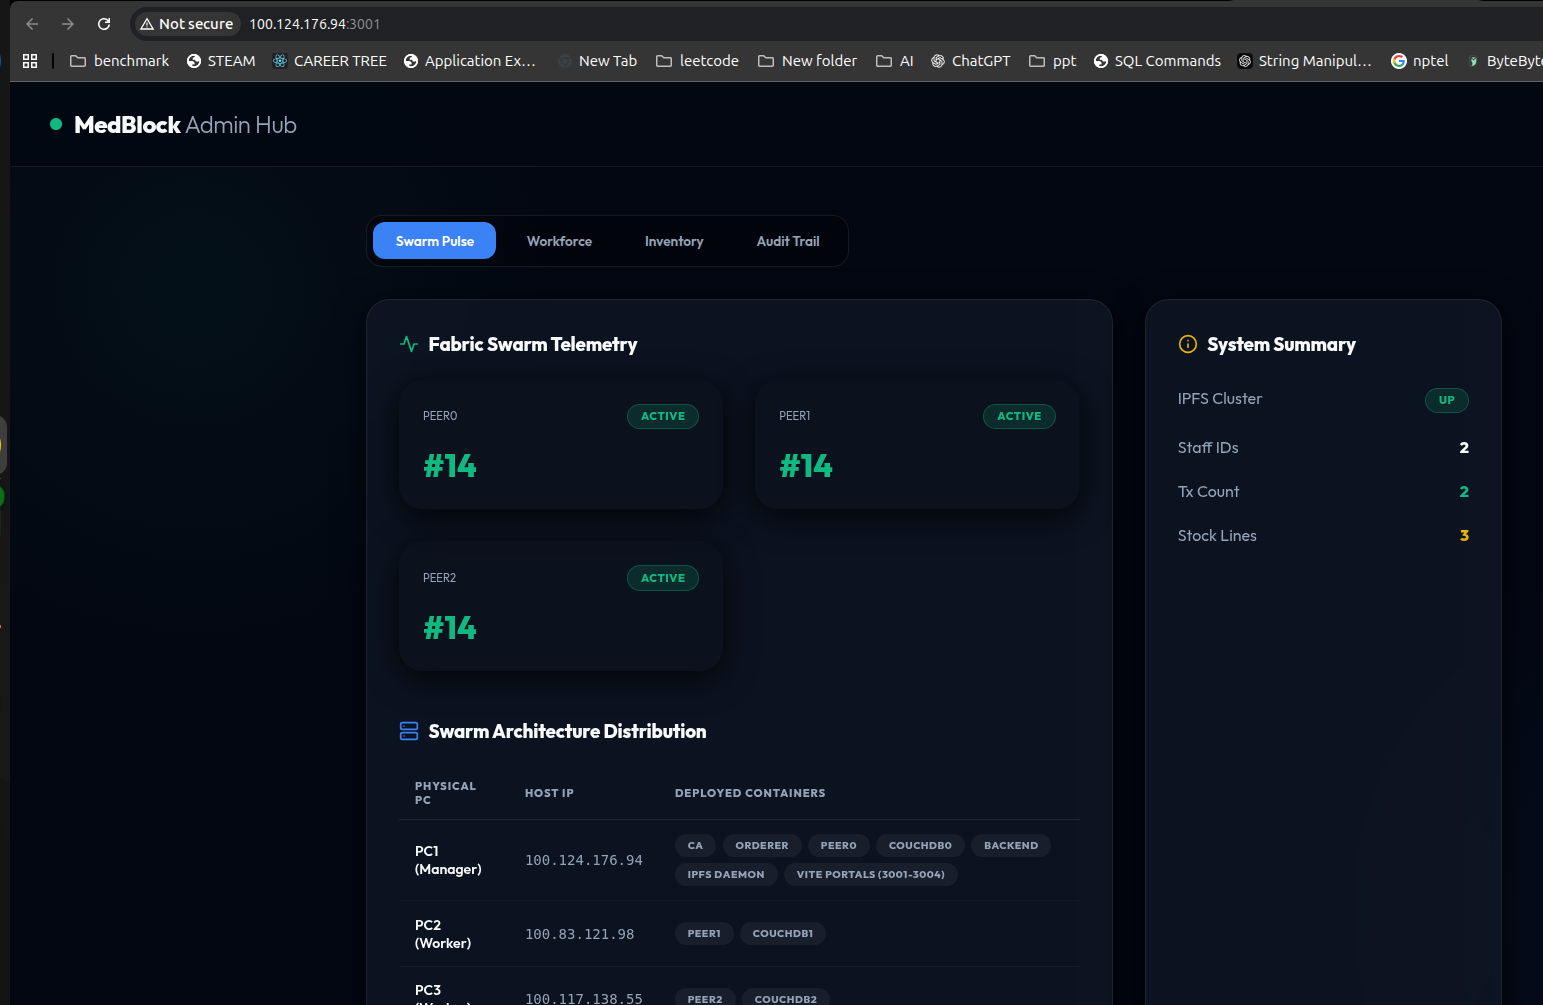
\includegraphics[width=0.9\textwidth]{images/dash-board.png}
    \caption{Manager Portal: Dashboard and Component Overview}
    \label{fig:manager_dashboard}
\end{figure}

\textbf{2. Registering a New Employee:}
\begin{enumerate}
    \item The Hospital Admin logs into the Manager Portal using their secure administrative credentials.
    \item Navigates to the ``Workforce Registry'' tab on the side-menu interface.
    \item Enters the employee's details (Staff ID, Full Name) and selects the specific Role (\texttt{doctor}, \texttt{pharmacist}, or \texttt{inventory}).
    \item Upon clicking ``Register'', the React frontend submits a POST request to the API Gateway.
    \item The Gateway bridges to the blockchain, invoking the \texttt{registerEmployee} smart contract function.
    \item The identity and role are permanently written into CouchDB under the \texttt{EMP\_} namespace, and the Fabric CA provisions the employee's cryptographic wallet.
\end{enumerate}
\begin{figure}[h]
    \centering
    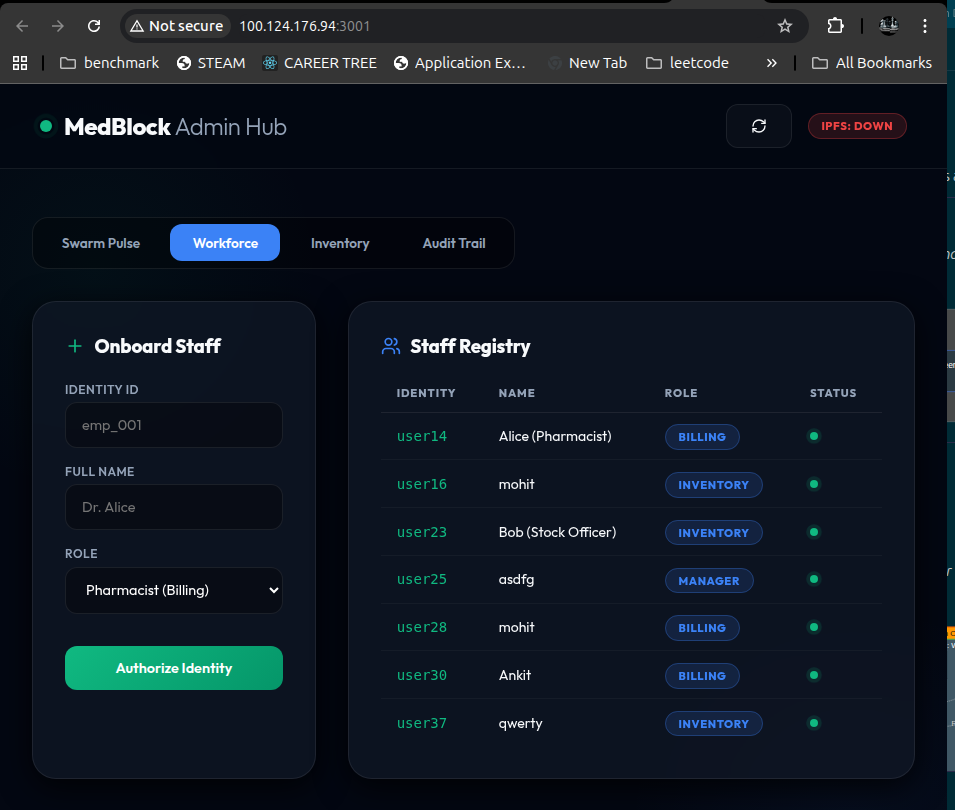
\includegraphics[width=0.9\textwidth]{images/workforce.png}
    \caption{Manager Portal: Employee Enrollment and Role Assignment}
    \label{fig:manager_register_emp}
\end{figure}

\textbf{3. Registering a New Patient:}
\begin{enumerate}
    \item The Admin navigates to the ``Patient Enrollment'' tab.
    \item Enters the patient's demographic details (National ID, Date of Birth).
    \item Submits the form, invoking the \texttt{createPatient} chaincode transaction.
    \item The ledger records the patient. Crucially, the system issues the patient a deterministic mapping to an X.509 Alias certificate, creating the cryptographic foundation for their self-sovereign identity access later.
\end{enumerate}

\textbf{4. Network Auditing and Block Monitoring:}
\begin{enumerate}
    \item Navigating to the ``Network Health'' tab fetches real-time ledger height metrics via the SDK, confirming that Gossip synchronization is functioning across PC1, PC2, and PC3.
    \item Navigating to the ``Global Audit'' tab allows the manager to pull all transparent hospital records. The chaincode executes a CouchDB Mango query across all \texttt{BILL\_} documents, giving administrators total oversight of activities.
\end{enumerate}
\begin{figure}[h]
    \centering
    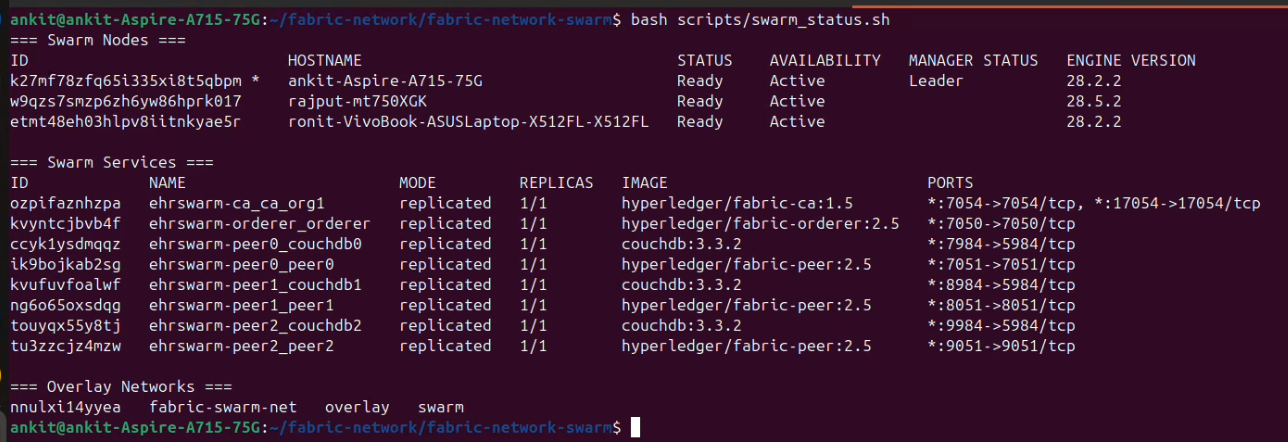
\includegraphics[width=0.9\textwidth]{images/status.png}
    \caption{Manager Portal: Swarm Network Health Monitoring}
    \label{fig:manager_network}
\end{figure}

\begin{figure}[h]
    \centering
    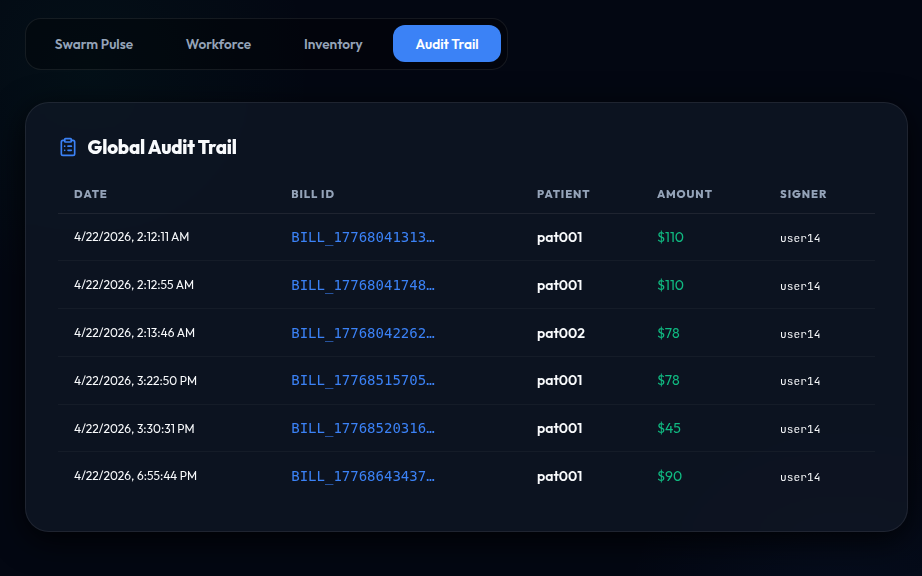
\includegraphics[width=0.9\textwidth]{images/audit.png}
    \caption{Manager Portal: Global Blockchain Audit Trail}
    \label{fig:manager_audit}
\end{figure}

\textbf{5. Hospital Inventory Oversight:}
\begin{enumerate}
    \item The manager can independently view global stock levels recorded on the ledger. 
    \item Accessing the ``Stock Monitor'' tab queries the \texttt{getAllInventory} chaincode, retrieving the immutable, real-time aggregated state of medicine quantities currently managed by the Inventory staff on PC3.
\end{enumerate}
\begin{figure}[h]
    \centering
    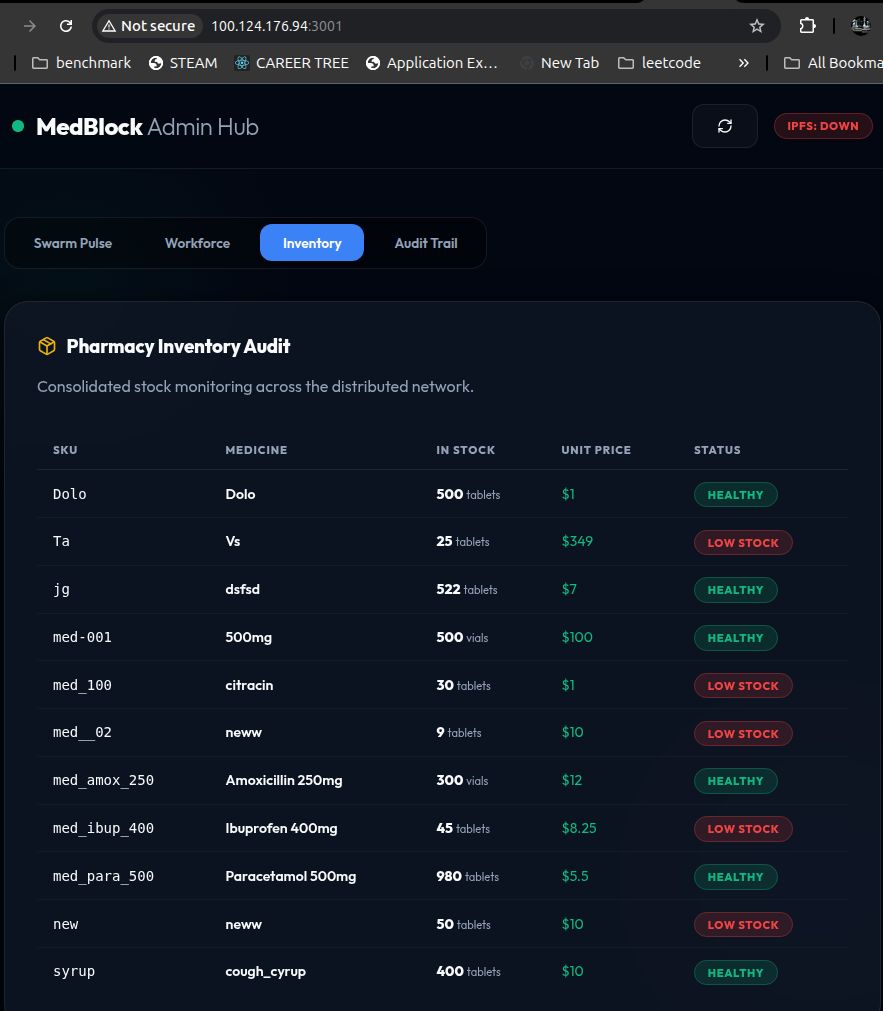
\includegraphics[width=0.9\textwidth]{images/inventory.png}
    \caption{Manager Portal: Read-Only Global Inventory Oversight}
    \label{fig:manager_inventory}
\end{figure}

\clearpage
%% ════════════════════════════════════════════════════════════════════════════
%% SECTION 2: MOHIT
%% ════════════════════════════════════════════════════════════════════════════

\section{Mohit Tomar (25CSM2R13): Smart Contract Lead \& Clinical Portals}

\subsection{Role Overview}
Mohit is responsible for the Fabric Chaincode (Smart Contracts) that define all business logic, the CouchDB state database on PC2, and the clinical-facing frontend applications (Patient Portal and Pharmacist/Billing Portal).

\subsection{Containers Hosted on PC2}

\begin{table}[h]
\centering
\caption{PC2 Container Inventory (Mohit Tomar)}
\label{tab:mohit_containers}
\begin{tabular}{|l|l|p{6cm}|}
\hline
\textbf{Container} & \textbf{Image} & \textbf{Purpose} \\
\hline
Peer1 & hyperledger/fabric-peer:2.5 & Endorsing peer for transaction simulation \\
\hline
CouchDB1 & couchdb:3.3.2 & State database with rich query support \\
\hline
Patient Portal & React (Vite) & Patient self-governance interface \\
\hline
Pharmacist Portal & React (Vite) & Prescription billing interface \\
\hline
\end{tabular}
\end{table}

\subsection{Smart Contract Architecture (Chaincode)}

The EHR chaincode is implemented in Node.js using the \texttt{fabric-contract-api} library. It manages four distinct asset types on the ledger:

\begin{table}[h]
\centering
\caption{Chaincode Asset Types}
\label{tab:asset_types}
\begin{tabular}{|l|l|l|p{4.5cm}|}
\hline
\textbf{Asset} & \textbf{Key Prefix} & \textbf{docType} & \textbf{Description} \\
\hline
Employee & \texttt{EMP\_} & employee & Hospital staff identity records \\
\hline
Patient & \texttt{PATIENT\_} & patient & Patient demographic and history \\
\hline
Bill & \texttt{BILL\_} & bill & Prescriptions and billing records \\
\hline
Inventory & \texttt{INV\_} & inventory & Medicine stock tracking \\
\hline
\end{tabular}
\end{table}

\textbf{Key File:} \texttt{chaincode/ehr/index.js}

\subsection{Identity Resolution Algorithm}

A critical component of the chaincode is the \texttt{\_getRole()} function, which determines the caller's role through a multi-step resolution process:

\begin{algorithm}[H]
\caption{Identity Resolution and Role Detection}
\label{alg:identity}
\begin{algorithmic}[1]
\Procedure{GetRole}{$ctx$}
    \State $role \gets$ \Call{GetCertAttribute}{$ctx$, ``role''}
    \If{$role \neq null$}
        \State \Return $role$ \Comment{Explicit CA attribute}
    \EndIf
    \State $id \gets$ \Call{GetClientID}{$ctx$}
    \If{$id$ contains ``admin'' or ``manager''}
        \State \Return ``manager''
    \EndIf
    \State $alias \gets$ \Call{ExtractCN}{$id$} \Comment{Extract Common Name from X.509 DN}
    \State $empData \gets$ \Call{GetState}{``EMP\_'' + $alias$}
    \If{$empData \neq null$ \textbf{and} $empData.isActive$}
        \State \Return $empData.role$ \Comment{Ledger-based registry lookup}
    \EndIf
    \State $patientLookup \gets$ \Call{GetState}{``ALIAS\_'' + $alias$ + ``\_PATIENT''}
    \If{$patientLookup \neq null$}
        \State \Return ``patient'' \Comment{Reverse alias patient lookup}
    \EndIf
    \State \Return ``guest'' \Comment{Fallback: no permissions}
\EndProcedure
\end{algorithmic}
\end{algorithm}

\subsection{CouchDB Rich Queries}

By configuring \texttt{CORE\_LEDGER\_STATE\_STATEDATABASE=CouchDB} in the peer environment, Mohit enabled the chaincode to execute JSON-based (Mango) queries. This replaces the default LevelDB key-value lookups with indexed, attribute-based searches:

\begin{lstlisting}[language=JavaScript, caption={CouchDB Rich Query Example (Chaincode)}]
// Fetch all bills for a specific patient
async getPatientBills(ctx, patientId) {
    const iterator = await ctx.stub.getStateByRange('', '');
    const results = [];
    while (true) {
        const result = await iterator.next();
        if (result.value) {
            const record = JSON.parse(result.value.value.toString());
            if (record.docType === 'bill' && record.patientId === patientId) {
                results.push(record);
            }
        }
        if (result.done) { await iterator.close(); break; }
    }
    return JSON.stringify(results);
}
\end{lstlisting}

\subsection{Patient Portal}

The Patient Portal embodies the concept of \textbf{Self-Sovereign Identity}. When a patient logs in, the system maps their physical ID to a deterministic X.509 certificate. The chaincode then ensures they can only access records where their \texttt{ownerAlias} matches.

\textbf{Key Features:}
\begin{itemize}
    \item View complete chronological medical history
    \item Download medical reports via IPFS CID hash retrieval
    \item Grant or revoke access to specific healthcare providers
    \item View list of entities currently authorized to access records
\end{itemize}

\textbf{Key File:} \texttt{app/patient/src/App.jsx}

\begin{figure}[h]
    \centering
    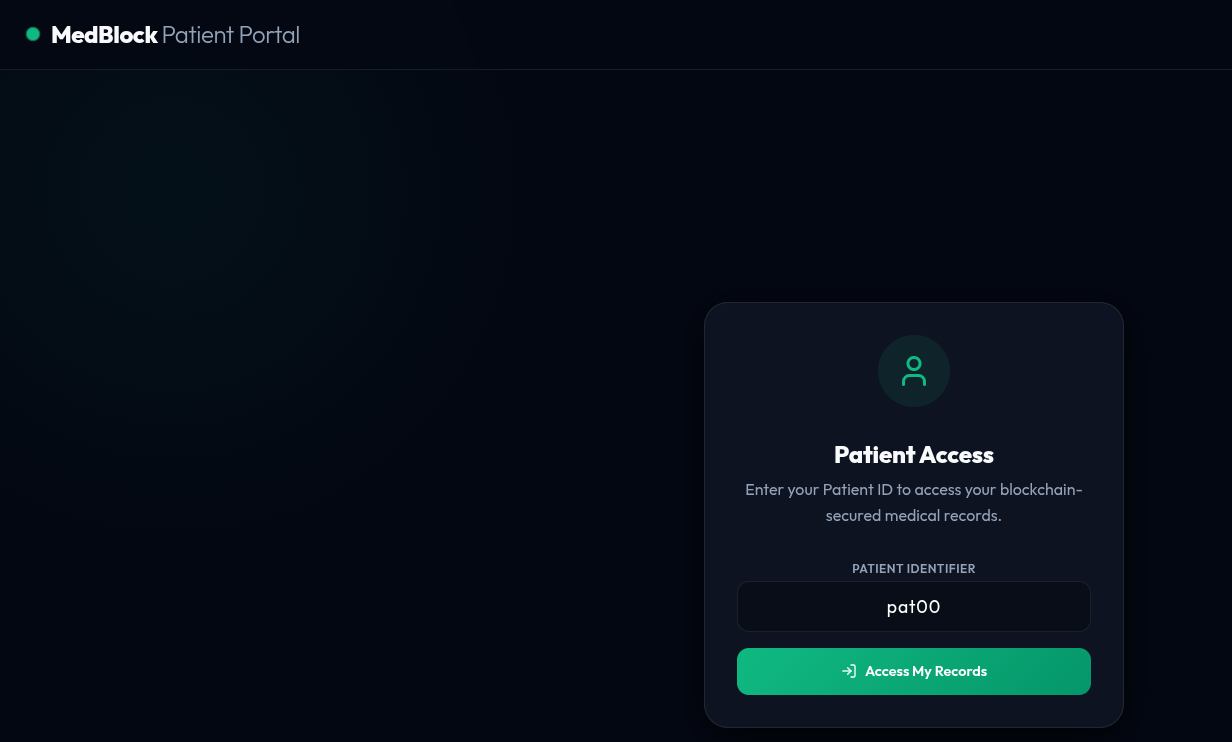
\includegraphics[width=1.0\textwidth]{images/patient_portal1.png}
    \caption{Patient Portal: Self-Sovereign Health Record Access (Part 1)}
    \label{fig:patient_portal1}
\end{figure}

\begin{figure}[h]
    \centering
    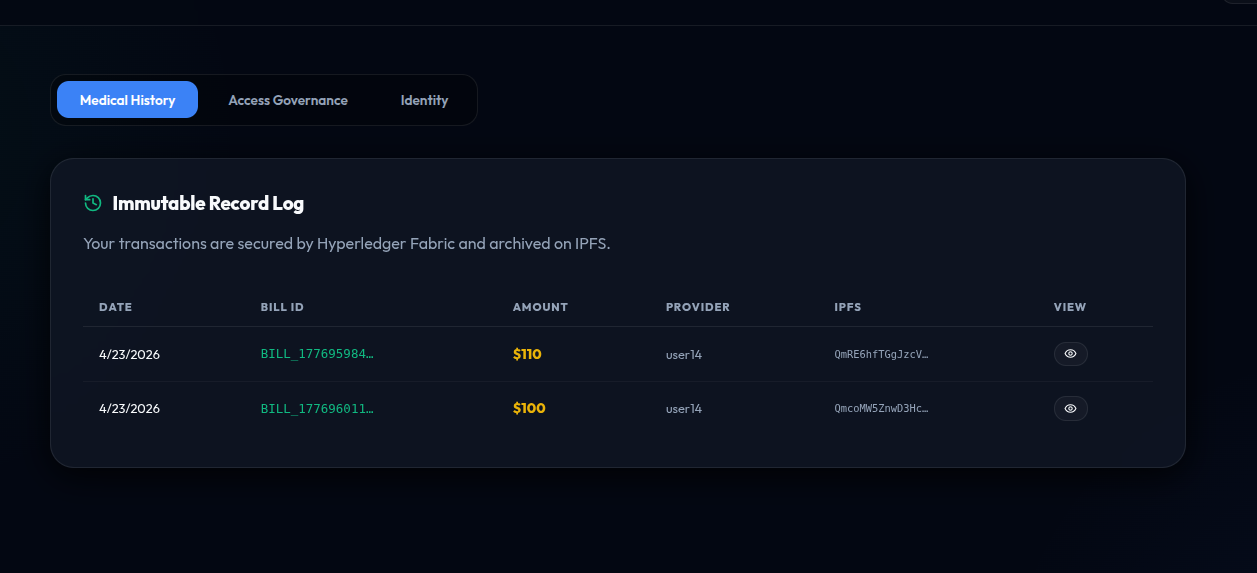
\includegraphics[width=1.0\textwidth]{images/patient_portal2.png}
    \caption{Patient Portal: Self-Sovereign Health Record Access (Part 2)}
    \label{fig:patient_portal2}
\end{figure}

\subsection{Pharmacist / Billing Portal}

The Pharmacist Portal demonstrates \textbf{Attribute-Based Access Control (ABAC)} in action. The chaincode verifies the caller's role and returns only prescription-relevant data (medicine names and quantities), explicitly filtering out private primary diagnoses.

\begin{algorithm}[H]
\caption{Billing Transaction with IPFS Anchoring}
\label{alg:billing}
\begin{algorithmic}[1]
\Procedure{ProcessBilling}{$patientId$, $medicineList$}
    \State Validate patient exists on ledger
    \State $doc \gets$ Build prescription document (medicines, doses, timestamps)
    \State $ipfsHash \gets$ \Call{UploadToIPFS}{$doc$} \Comment{Off-chain storage}
    \State $billId \gets$ Generate unique bill identifier
    \State \Call{InvokeChaincode}{``createBill'', $billId$, $patientId$, $ipfsHash$}
    \For{each $medicine$ in $medicineList$}
        \If{$medicine.itemId$ exists}
            \State \Call{InvokeChaincode}{``deductInventoryItem'', $medicine.itemId$, $quantity$}
        \EndIf
    \EndFor
    \State \Return success with $billId$ and $ipfsHash$
\EndProcedure
\end{algorithmic}
\end{algorithm}

\textbf{Key File:} \texttt{app/billing/src/App.jsx}

\begin{figure}[h]
    \centering
    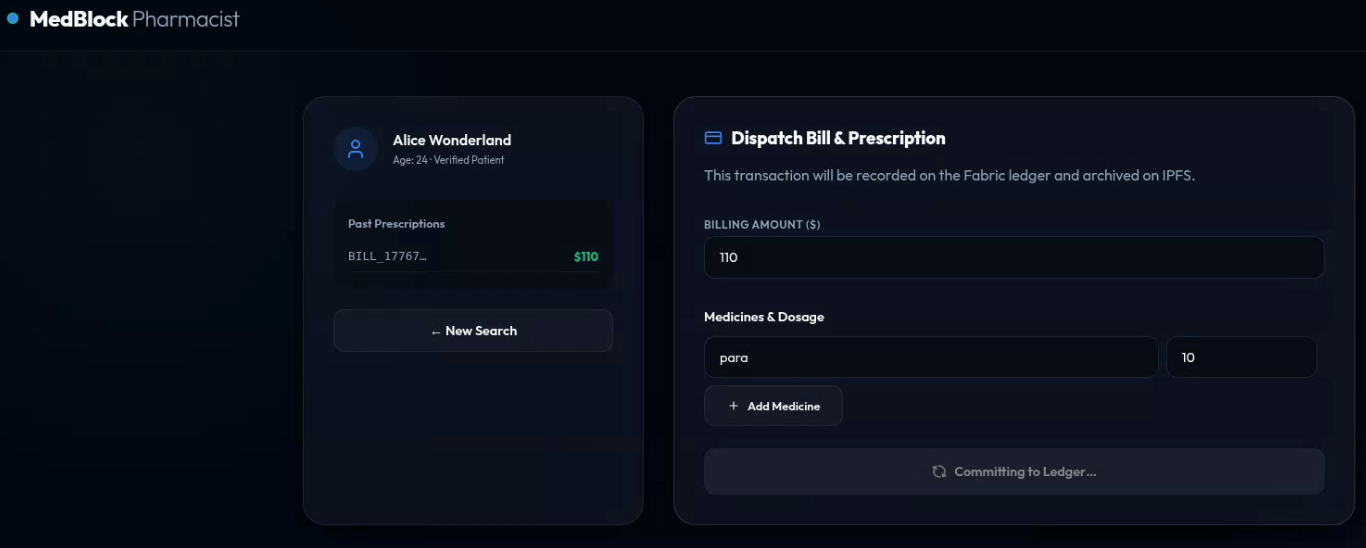
\includegraphics[width=1.0\textwidth]{images/pharma_portal1.png}
    \caption{Pharmacist Portal: Prescription Fulfillment and Billing Interface (Part 1)}
    \label{fig:pharmacist_portal1}
\end{figure}

\begin{figure}[h]
    \centering
    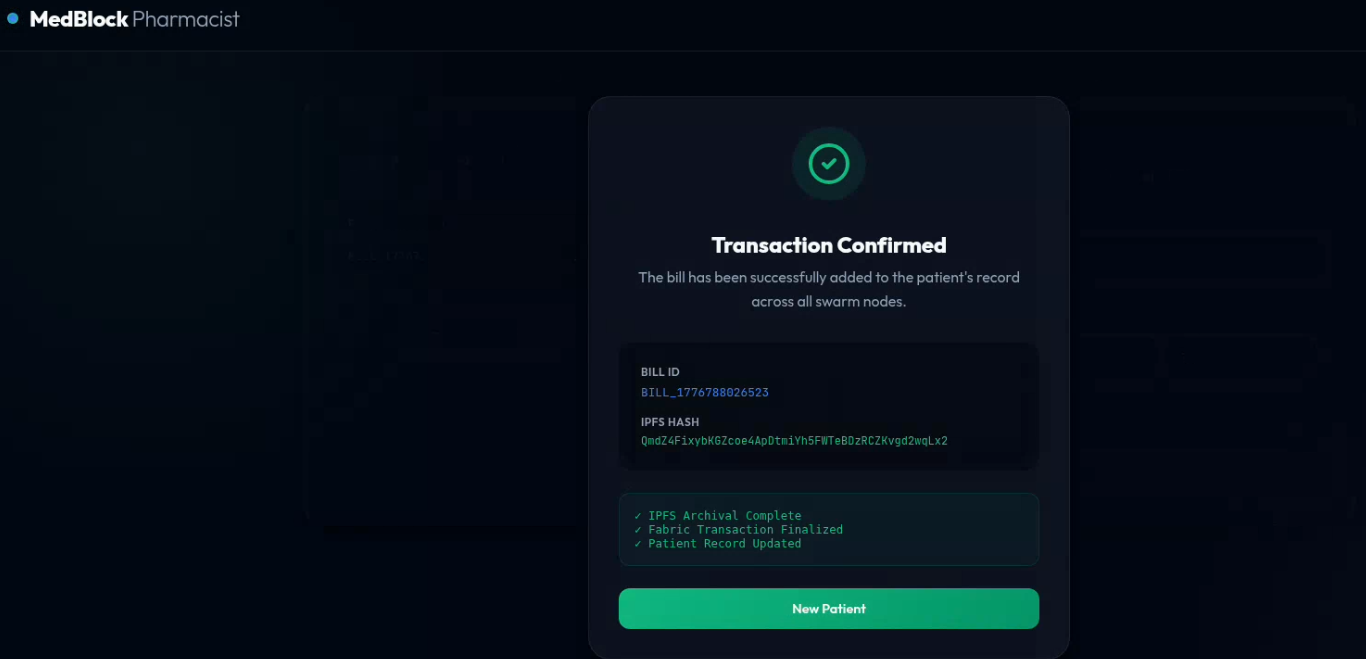
\includegraphics[width=1.0\textwidth]{images/pharma_portal2.png}
    \caption{Pharmacist Portal: Prescription Fulfillment and Billing Interface (Part 2)}
    \label{fig:pharmacist_portal2}
\end{figure}

\clearpage
%% ════════════════════════════════════════════════════════════════════════════
%% SECTION 3: RONIT
%% ════════════════════════════════════════════════════════════════════════════

\section{Ronitsingh Rawat (25CSM2S06): API Gateway Architect \& Inventory Lead}

\subsection{Role Overview}
Ronit is responsible for the Node.js API Gateway that bridges the React frontends to the blockchain via the Fabric SDK, the FileSystemWallet management, and the complete Inventory Application. He operates PC3, ensuring high availability and fault tolerance.

\subsection{Containers Hosted on PC3}

\begin{table}[h]
\centering
\caption{PC3 Container Inventory (Ronitsingh Rawat)}
\label{tab:ronit_containers}
\begin{tabular}{|l|l|p{6cm}|}
\hline
\textbf{Container} & \textbf{Image} & \textbf{Purpose} \\
\hline
Peer2 & hyperledger/fabric-peer:2.5 & Redundancy peer for fault tolerance \\
\hline
CouchDB2 & couchdb:3.3.2 & Mirrored state database \\
\hline
API Gateway & Node.js (Express) & Fabric SDK bridge (REST $\to$ gRPC) \\
\hline
Inventory Portal & React (Vite) & Medicine supply chain tracking \\
\hline
\end{tabular}
\end{table}

\subsection{API Gateway Architecture}

The API Gateway (\texttt{app/backend/app.js}) is the central nervous system of the Electronic Health Record (EHR) System. It translates standard HTTP/REST requests from the React frontends into cryptographically signed gRPC transactions using the \texttt{fabric-network} SDK.

\textbf{Core Dependencies:}
\begin{itemize}
    \item \texttt{fabric-network} — Official Hyperledger Fabric SDK for Node.js
    \item \texttt{express} — HTTP REST framework
    \item \texttt{axios} — IPFS API communication
    \item \texttt{crypto} — Deterministic identity hashing
\end{itemize}

\subsection{Smart Routing Algorithm}

A unique feature of the API Gateway is its intelligent transaction routing. Instead of sending all requests to a single peer, the gateway distributes load across the Swarm:

\begin{algorithm}[H]
\caption{Smart Transaction Routing}
\label{alg:routing}
\begin{algorithmic}[1]
\Procedure{SmartRoute}{$functionName$, $endorsers$}
    \State $module \gets$ \Call{ClassifyFunction}{$functionName$}
    \If{$module$ = ``billing'' \textbf{and} $|endorsers| > 1$}
        \State $targetPeer \gets endorsers[1]$ \Comment{Route to Peer1 (PC2)}
    \ElsIf{$module$ = ``inventory'' \textbf{and} $|endorsers| > 2$}
        \State $targetPeer \gets endorsers[2]$ \Comment{Route to Peer2 (PC3)}
    \Else
        \State $targetPeer \gets endorsers[0]$ \Comment{Default to Peer0 (PC1)}
    \EndIf
    \State \Return $targetPeer$
\EndProcedure
\end{algorithmic}
\end{algorithm}

\subsection{Wallet and Identity Management}

The API manages a \texttt{FileSystemWallet} containing X.509 certificates for all registered users. When a frontend request arrives, the gateway:

\begin{enumerate}
    \item Extracts the user ID from the request body.
    \item Hashes the ID deterministically to map it to one of 50 pre-enrolled certificates (\texttt{user1} through \texttt{user50}).
    \item Loads the corresponding private key from the wallet.
    \item Creates a Gateway connection using the loaded identity.
    \item Signs and submits the transaction to the target peer.
\end{enumerate}

\begin{lstlisting}[language=JavaScript, caption={Identity Mapping Function (app.js)}]
function mintUserCertificate(id) {
    if (!id) return 'user1';
    if (id === 'admin' || id === 'manager') return 'admin';
    const hash = crypto.createHash('sha256').update(id).digest('hex');
    const index = (parseInt(hash.slice(0, 8), 16) % 50) + 1;
    return `user${index}`;
}
\end{lstlisting}

\subsection{High Availability and Peer Redundancy}

PC3 hosts Peer2, which serves as a redundancy node. Its importance lies in:

\begin{itemize}
    \item \textbf{Fault Tolerance:} If Mohit's PC2 goes offline, the API Gateway reroutes transactions to Peer2, ensuring zero downtime.
    \item \textbf{State Mirroring:} CouchDB2 maintains an exact replica of the world state through the Gossip protocol.
    \item \textbf{Independent Validation:} Peer2 independently validates all blocks received from the Orderer, ensuring no single peer can forge false transactions.
\end{itemize}

\begin{figure}[h]
    \centering
    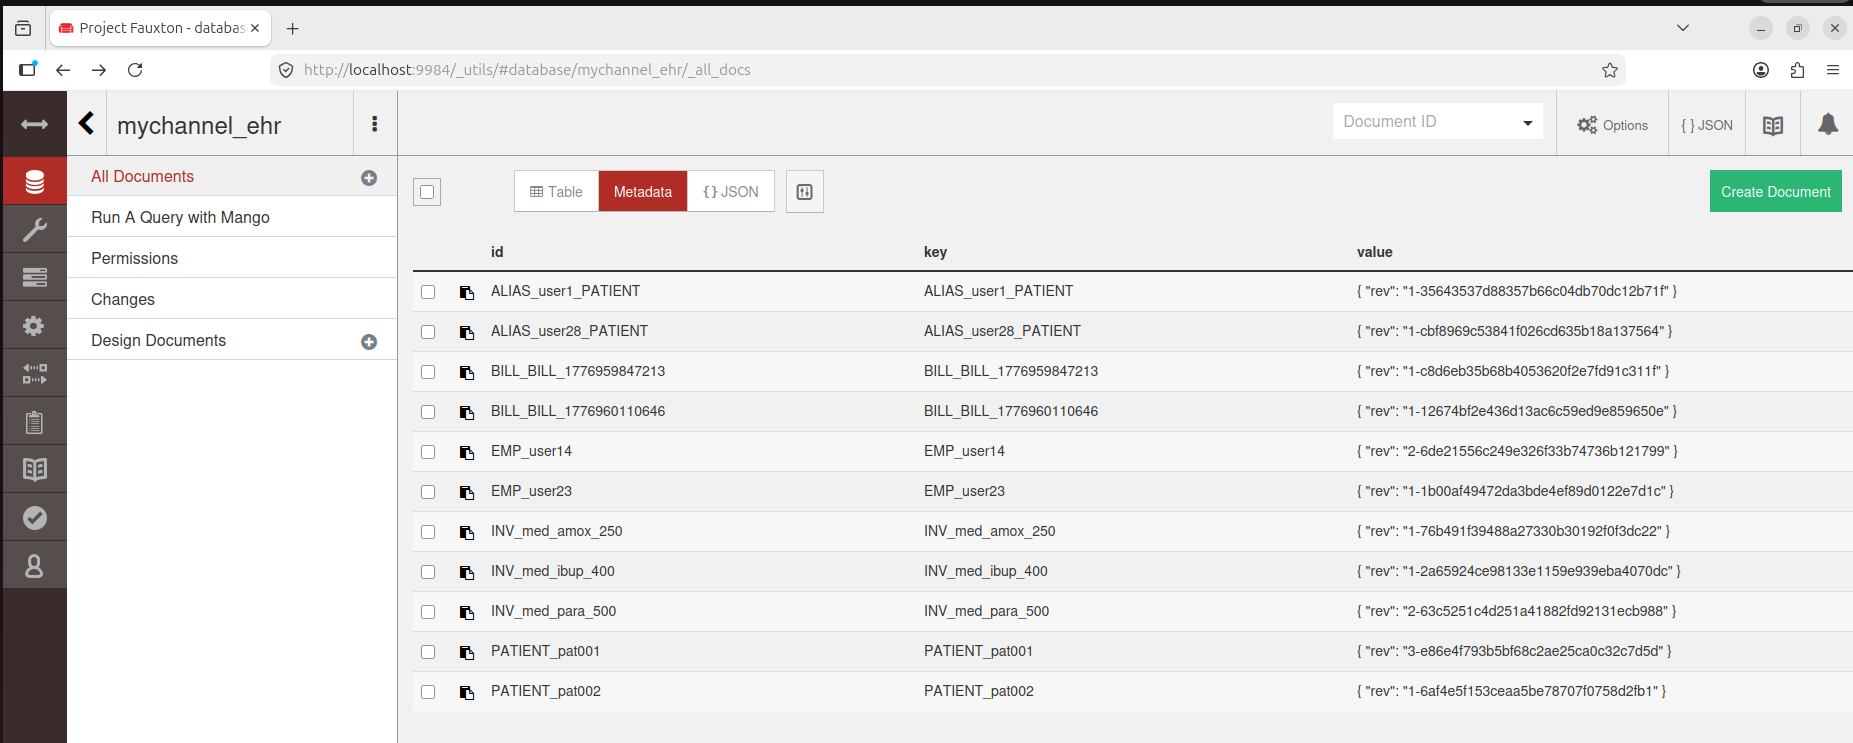
\includegraphics[width=0.9\textwidth]{images/couchdb.png}
    \caption{State Mirroring: CouchDB2 Interface on PC3}
    \label{fig:couchdb_mirror}
\end{figure}

\subsection{Inventory Application}

The Inventory Application extends the EHR platform into the hospital supply chain. It tracks medicine stock as digital assets on the Fabric ledger.

\begin{algorithm}[H]
\caption{Inventory Deduction with Fraud Prevention}
\label{alg:inventory}
\begin{algorithmic}[1]
\Procedure{DeductInventory}{$itemId$, $quantity$}
    \State $role \gets$ \Call{GetRole}{$ctx$}
    \If{$role \notin$ \{``manager'', ``billing'', ``inventory''\}}
        \State \textbf{throw} ``Access Denied''
    \EndIf
    \State $item \gets$ \Call{GetState}{``INV\_'' + $itemId$}
    \If{$item = null$}
        \State \textbf{throw} ``Item not found''
    \EndIf
    \If{$item.quantity < quantity$}
        \State \textbf{throw} ``Insufficient stock''
    \EndIf
    \State $item.quantity \gets item.quantity - quantity$
    \State $item.lastDeducted \gets$ current timestamp
    \State \Call{PutState}{``INV\_'' + $itemId$, $item$}
    \State \Return $item$
\EndProcedure
\end{algorithmic}
\end{algorithm}

\textbf{Key Feature — Atomic Billing-Inventory Linkage:} When a pharmacist fulfills a prescription through the Billing Portal, the API Gateway atomically triggers an \texttt{invokeChaincode(`deductInventoryItem')} call. Because the blockchain is immutable, it is mathematically impossible for medicine to be dispensed without the ledger permanently recording the stock deduction.

\begin{figure}[h]
    \centering
    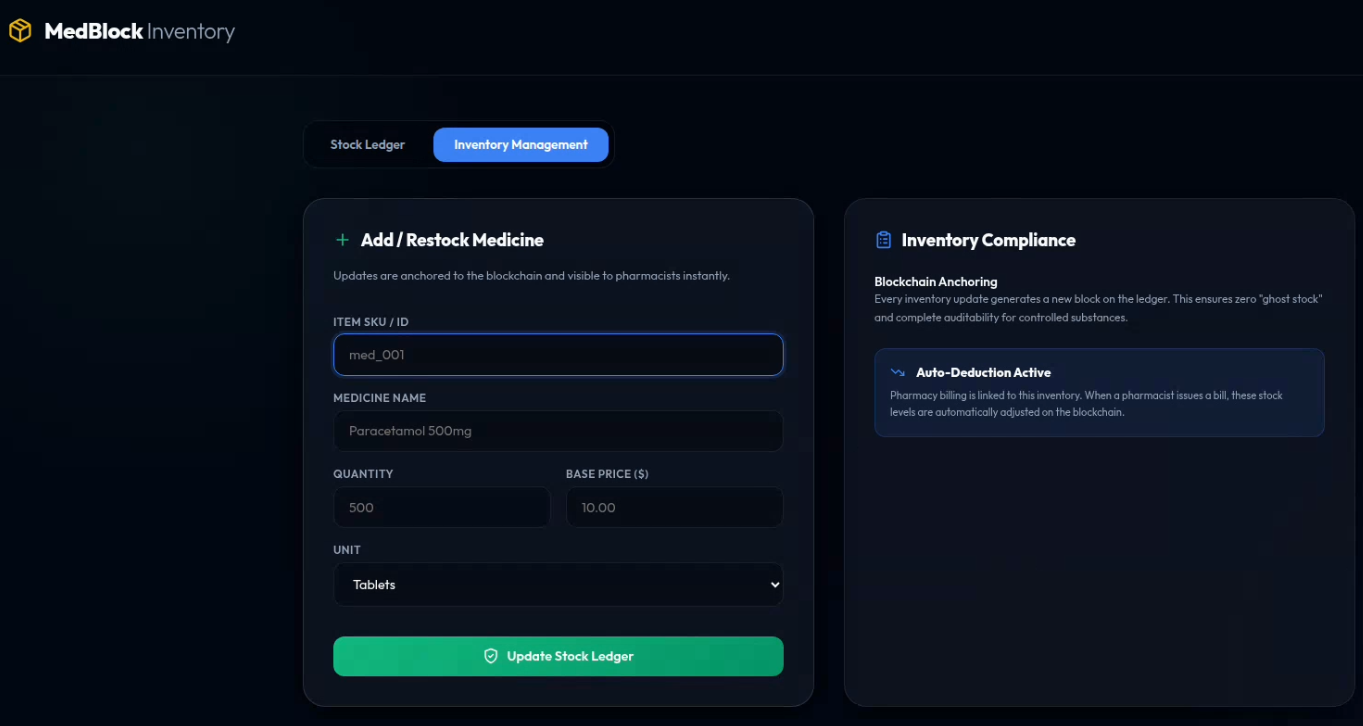
\includegraphics[width=0.9\textwidth]{images/inventory1.png}
    \caption{Inventory Portal: Adding New Medicine Stock to the Ledger}
    \label{fig:inventory_portal1}
\end{figure}

\begin{figure}[h]
    \centering
    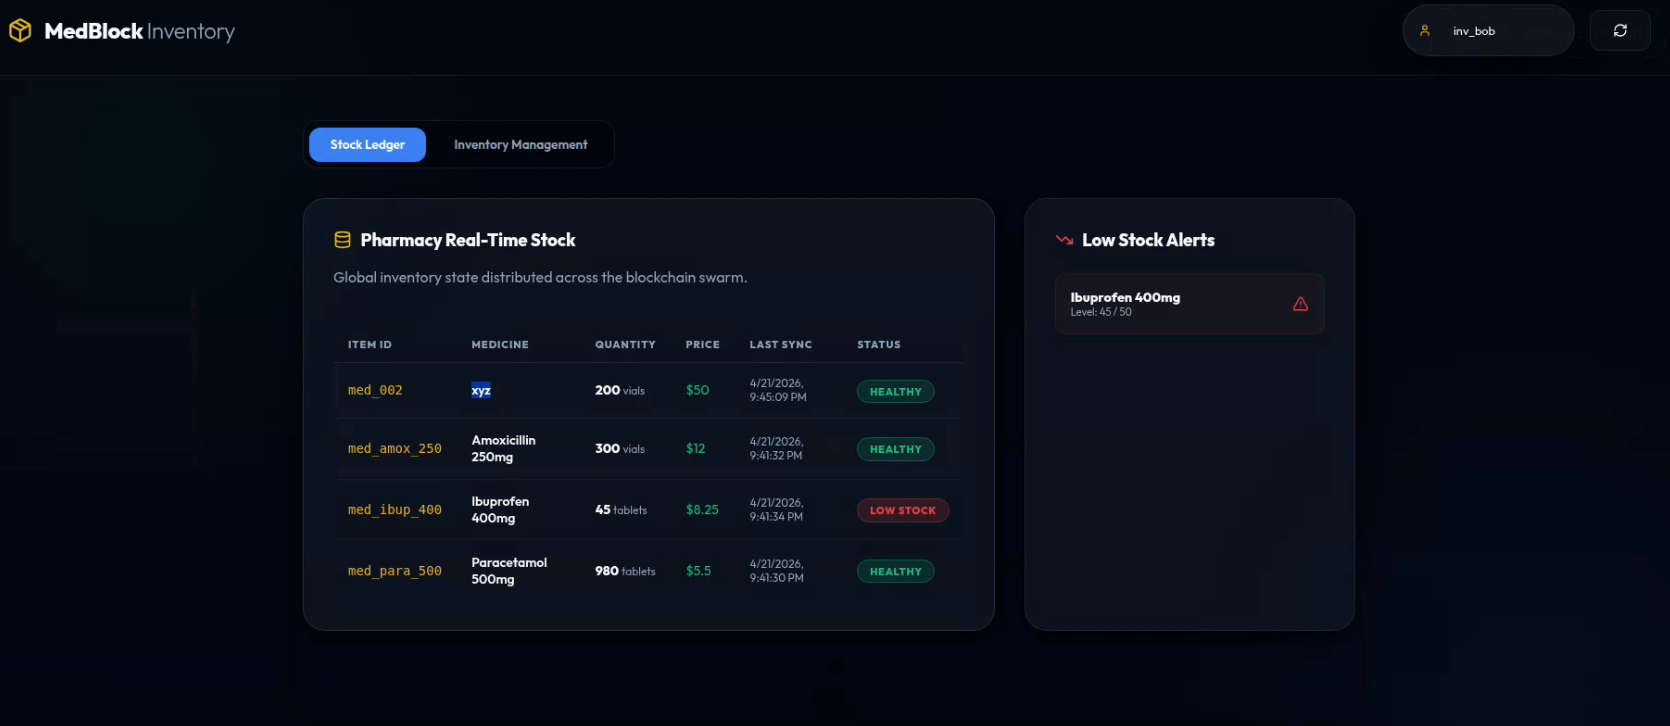
\includegraphics[width=0.9\textwidth]{images/inventory2.png}
    \caption{Inventory Portal: Medicine Stock Management and Deduction View}
    \label{fig:inventory_portal2}
\end{figure}

\clearpage
%% ════════════════════════════════════════════════════════════════════════════
%% SECTION 4: VERIFICATION AND RESULTS
%% ════════════════════════════════════════════════════════════════════════════

\section{Verification and Results}

\subsection{Ledger Synchronization Verification}

To verify that the Gossip protocol successfully synchronizes data across all three nodes, the following diagnostic commands were executed on each PC:

\begin{lstlisting}[language=bash, caption={Block Height Verification on All Peers}]
# On PC1 (Ankit):
docker exec $(docker ps -q -f name=peer0) \
  peer channel getinfo -c mychannel

# On PC2 (Mohit):
docker exec $(docker ps -q -f name=peer1) \
  peer channel getinfo -c mychannel

# On PC3 (Ronit):
docker exec $(docker ps -q -f name=peer2) \
  peer channel getinfo -c mychannel
\end{lstlisting}

All three peers reported identical block heights and matching \texttt{currentBlockHash} values, confirming perfect ledger synchronization across the distributed Swarm network.

\subsection{CouchDB State Verification}

Direct CouchDB queries on each node confirmed that the world state was replicated correctly:

\begin{lstlisting}[language=bash, caption={CouchDB State Query on Worker Nodes}]
# On PC2 (Mohit):
docker exec $(docker ps -q -f name=couchdb1) \
  curl -s -u admin:adminpw http://localhost:5984/mychannel_ehr/_all_docs

# On PC3 (Ronit):
docker exec $(docker ps -q -f name=couchdb2) \
  curl -s -u admin:adminpw http://localhost:5984/mychannel_ehr/_all_docs
\end{lstlisting}


\subsection{System Specifications}

\begin{table}[h]
\centering
\caption{Development and Deployment Environment}
\label{tab:system_specs}
\begin{tabular}{|l|l|}
\hline
\textbf{Component} & \textbf{Specification} \\
\hline
Hyperledger Fabric & v2.5 (LTS) \\
\hline
Docker Engine & v24.x \\
\hline
Docker Swarm & Native orchestration \\
\hline
Node.js & v18.x LTS \\
\hline
React & v18.x (Vite build) \\
\hline
CouchDB & v3.3.2 \\
\hline
IPFS & Kubo v0.18+ \\
\hline
VPN & Tailscale (WireGuard) \\
\hline
Operating System & Ubuntu 22.04 LTS \\
\hline
\end{tabular}
\end{table}
